\documentclass[12pt]{article}

\usepackage{sbc-template}

\usepackage{graphicx}
\usepackage{float}
\usepackage{url}
\usepackage{hyperref}

\usepackage[brazil]{babel}   
\usepackage[utf8]{inputenc}

% \usepackage[a4paper,top=1.1cm,bottom=2.1cm,left=2.5cm,right=2.5cm]{geometry}

\usepackage{lmodern,booktabs,tabularx,array,caption,hyperref,microtype,placeins,titling}

\setlength{\droptitle}{-1.5cm}
\hypersetup{hidelinks}
\urlstyle{same}
\setlength{\parindent}{1.25cm}
\setlength{\parskip}{1pt}
\setlength{\emergencystretch}{2em}
\captionsetup{font=small,labelfont=bf}

\graphicspath{{./images/}}

\sloppy

\title{Previsão horária de geração de energia fotovoltaica utilizando redes LSTM e restrições físicas: um estudo comparativo em cenário simulado de Pernambuco}


% André Luiz de Santana Silva - 01837755

% Enio Enrique Santiago da Silva - 01851994

% Fernando Vitor Miguel Baracho - 01845646
% João Gabriel Batista Viana Muniz - 01802624
% Érico André da Silva - 01123361
% Jadilson Rodrigues Ferreira - 01826199

\author{
André Luiz de Santana,
    \href{http://lattes.cnpq.br/0529785947460222}{SILVA, E. A.} \inst{1},
    João Gabriel Batista\\
    Jadilson Rodrigues, 
    Fernando Vitor Miguel,
    Enio Enrique Santiago,
}

\address{Análise e Desenvolvimento de Sistemas \\Paulista -- PE -- Brasil
}
\date{2026}

\begin{document}
\maketitle
% \noindent\textbf{Abstract.} Photovoltaic generation varies with solar radiation, weather conditions and system characteristics. This study evaluates Long Short-Term Memory (LSTM) networks for one-hour-ahead energy forecasting in a hypothetical 5.5 kWp system in Recife, Brazil. Experiments used 120 days of synthetic data and simulated weather forecast errors. Direct LSTM with Huber loss achieved a test MAE of 0.0572 kWh, WAPE of 6.89\%, and R-squared of 0.9910. Residual LSTM reduced the physical baseline MAE by 28.47\%. Results demonstrate proof-of-concept feasibility, not validated accuracy on measured generation.
\\\\
\noindent\textbf{Keywords:} photovoltaic energy; machine learning; time series; LSTM; weather forecasting.\\
\begin{resumo} 
A geração de energia fotovoltaica varia conforme a disponibilidade de radiação solar, as condições meteorológicas e as características da instalação. Este trabalho avalia o uso de redes neurais recorrentes do tipo Long Short-Term Memory (LSTM) para estimar a energia gerada na próxima hora. Foi desenvolvida uma prova de conceito para um sistema hipotético de 5,5 kWp, com inversor de 5 kW, localizado em Recife, Pernambuco. Os experimentos utilizaram 120 dias de dados sintéticos, com perturbações meteorológicas simuladas, e compararam o LSTM direto, o LSTM residual, a RNN simples, o Random Forest e métodos de referência. O LSTM direto com perda de Huber apresentou o menor erro no teste, com MAE de 0,0572 kWh, WAPE de 6,89\% e coeficiente de determinação de 0,9910. O LSTM residual reduziu em 28,47\% o MAE da referência física. Os resultados demonstram o potencial da abordagem como protótipo acadêmico.
\\\\
\noindent\textbf{Palavras-chave:} energia solar fotovoltaica; aprendizado de máquina; séries temporais; LSTM; previsão meteorológica.

\end{resumo}
\section{Introdução}
A energia solar fotovoltaica contribui para a diversificação das fontes energéticas. Entretanto, sua produção não é constante: varia conforme a posição do Sol, a presença de nuvens, a temperatura e as características dos equipamentos. Essa variabilidade dificulta o planejamento energético, especialmente quando a geração deve acompanhar a demanda ou auxiliar a operação da rede elétrica.

Corrêa (2026) \cite{correa} destaca a importância de combinar informações meteorológicas e séries históricas para estimar a produção futura de uma instalação fotovoltaica. Em seu estudo, realizado com dados diários de geração do IFES -- Campus Linhares, a inclusão de variáveis climáticas e componentes sazonais contribuiu para melhorar o desempenho da rede LSTM. A investigação constitui uma referência teórica e metodológica para este projeto, cujo objetivo é diferente: avaliar a previsão horária em um cenário simulado de Pernambuco.

O objetivo geral é desenvolver e comparar modelos de aprendizado de máquina capazes de estimar a geração da próxima hora, considerando o histórico de energia, a meteorologia e os limites físicos de um sistema fotovoltaico. Como objetivos específicos, busca-se incorporar os parâmetros dos módulos e do inversor, avaliar o LSTM direto e residual e comparar seus erros com os de modelos mais simples. Não se pretende provar previamente que uma rede neural seja superior a todos os demais métodos.

\section{Fundamentação teórica}
\subsection{Energia solar e radiação incidente}
A energia solar pode ser aproveitada para produzir calor ou eletricidade. A disponibilidade do recurso solar na superfície terrestre não depende apenas da posição geográfica: a rotação da Terra, o ciclo anual e os fenômenos atmosféricos modificam a quantidade de energia recebida ao longo do tempo. Parte da radiação é absorvida, refletida ou espalhada antes de chegar ao solo, conforme a descrição de Corrêa (2026, p. 18--20) \cite{correa}.

É importante distinguir irradiância de irradiação. A primeira indica a potência da radiação por unidade de área, geralmente expressa em W/m\textsuperscript{2}. A segunda representa a energia acumulada nessa área durante determinado intervalo, expressa, por exemplo, em Wh/m\textsuperscript{2}. Para caracterizar o recurso solar, utilizam-se três componentes principais: a irradiância global horizontal (GHI), que representa a radiação total recebida por uma superfície horizontal; a irradiância normal direta (DNI), associada aos raios solares que chegam diretamente; e a irradiância horizontal difusa (DHI), decorrente do espalhamento atmosférico. A radiação refletida pelo entorno também pode contribuir para a energia incidente em módulos inclinados.

Essas informações são relevantes porque a potência produzida pelos módulos depende da radiação que efetivamente alcança sua superfície. A mesma irradiância horizontal pode resultar em diferentes níveis de geração quando se alteram a inclinação, a orientação ou a posição do Sol.

\subsection{Sistemas fotovoltaicos e fatores de desempenho}
As células fotovoltaicas convertem a radiação solar em eletricidade por meio do efeito fotovoltaico. A associação de células forma os módulos, cuja conexão permite construir instalações com diferentes potências. Os módulos geram corrente contínua (CC), enquanto o inversor realiza a conversão para corrente alternada (CA), adequada ao consumo e à conexão com a rede elétrica \cite{correa}.

A potência nominal dos módulos, expressa em watts-pico (Wp), é determinada em condições padronizadas de ensaio. Ela não representa uma produção constante ao longo do dia. A energia, por sua vez, é medida em quilowatt-hora (kWh), e corresponde à potência acumulada durante um intervalo. Assim, um inversor limitado a 5 kW pode entregar, no modelo adotado, no máximo 5 kWh em uma hora.

A irradiância é o principal fator de geração, porém a temperatura das células também modifica a eficiência de conversão. Em módulos convencionais, o aumento da temperatura tende a reduzir a potência elétrica disponível para a mesma irradiância. A ventilação pode auxiliar no resfriamento dos módulos, enquanto a nebulosidade altera a quantidade e a composição da radiação que alcança as placas. A chuva e a umidade podem estar associadas às condições atmosféricas que influenciam a geração, mas seus efeitos não são necessariamente independentes da irradiância.

O inversor também impõe restrições. Quando a potência disponível do arranjo ultrapassa o limite de conversão, a saída é limitada à capacidade do equipamento, fenômeno denominado \textit{clipping}. Além disso, existem perdas na conversão e nos componentes elétricos. Por isso, considerar somente o clima, sem representar os equipamentos, pode levar a estimativas inconsistentes com a instalação analisada.

\subsection{Previsão de geração e aprendizado de máquina}
Segundo Corrêa (2026, p. 21--23) \cite{correa}, as técnicas de previsão podem ser organizadas em abordagens físicas, estatísticas e híbridas. Os modelos físicos representam fenômenos como a posição solar, a incidência de radiação e a conversão de energia. Já os métodos estatísticos e de aprendizado de máquina extraem relações dos dados históricos. As abordagens híbridas combinam conhecimentos físicos com modelos que aprendem a partir de exemplos.

Neste projeto, o aprendizado de máquina é tratado como um problema de regressão supervisionada: o algoritmo recebe informações de entrada e aprende a estimar uma variável numérica, a energia fotovoltaica em kWh. A qualidade das entradas e a separação adequada dos dados são tão importantes quanto a escolha do algoritmo. Um modelo complexo não garante, por si só, menor erro.

\subsection{Redes neurais recorrentes e LSTM}
As redes neurais artificiais utilizam conexões ponderadas para transformar informações de entrada em previsões. Durante o treinamento, os pesos são modificados de modo a reduzir a diferença entre os valores previstos e os valores-alvo. Em uma série temporal, a ordem das observações contém informação: a geração de uma hora pode estar relacionada às condições das horas anteriores.

As redes neurais recorrentes (RNN) incorporam um estado interno que é atualizado a cada passo da sequência. Entretanto, redes recorrentes simples podem ter dificuldade em preservar dependências temporais distantes devido a problemas na propagação do gradiente. A LSTM, proposta por Hochreiter e Schmidhuber (1997) \cite{lstm}, foi desenvolvida para facilitar o aprendizado dessas dependências.

De acordo com a descrição da célula LSTM apresentada por Corrêa (2026, p. 24--28) \cite{correa}, sua memória é regulada por três mecanismos principais. A porta de esquecimento controla a retenção de informações anteriores; a porta de entrada determina quais novas informações atualizam a memória; e a porta de saída define a parcela do estado interno utilizada na saída. Esses mecanismos possibilitam que a rede processe uma sequência sem tratar todos os registros anteriores como igualmente relevantes.

No contexto fotovoltaico, o LSTM pode aprender relações entre o histórico de geração, o ciclo diário e as variações meteorológicas. A escolha da arquitetura se justifica pela natureza sequencial dos dados, não pela garantia de superioridade sobre a RNN ou outros métodos. Neste estudo, emprega-se uma rede com uma camada LSTM de 32 unidades, suficiente para avaliar a proposta sem acrescentar complexidade desnecessária.

\subsection{Sazonalidade, Random Forest e aprendizagem residual}
A geração fotovoltaica apresenta padrões cíclicos associados ao dia e ao ano. A persistência sazonal é uma referência simples: prevê a geração repetindo o valor registrado no mesmo horário do dia anterior. Embora útil para comparação, pode falhar quando as condições atmosféricas mudam. A codificação cíclica do horário e do dia do ano, por outro lado, permite representar a proximidade temporal entre o final e o início de cada ciclo.

O Random Forest é um método que combina várias árvores de decisão, agregando suas previsões para estimar a variável-alvo \cite{rf}. Ele pode representar relações não lineares entre clima e geração sem utilizar uma memória recorrente interna. Para comparar os métodos, pode receber os mesmos registros históricos organizados como atributos.

A aprendizagem residual combina uma estimativa física com uma rede neural que aprende sua diferença em relação ao alvo. A previsão final é a soma da referência com a correção aprendida. A abordagem incorpora os conhecimentos sobre os equipamentos, mas depende da qualidade da referência e dos dados. Também foi avaliado um LSTM direto, que estima a geração sem essa correção explícita.
\section{Materiais e métodos}
\subsection{Instalação e conjunto de dados}
O sistema de referência é uma instalação hipotética conectada à rede elétrica em Recife, sem bateria ou gerador auxiliar. A Tabela~\ref{tab:cfg} apresenta os parâmetros configurados. Os valores de eficiência e perdas são hipóteses de simulação, não especificações verificadas de equipamentos reais.

\begin{table}[!ht]
\centering
\caption{Características do sistema fotovoltaico simulado}
\label{tab:cfg}
% \small
\begin{tabularx}{0.94\textwidth}{@{}Xl@{}}\toprule
Parâmetro & Valor\\\midrule
Quantidade e potência dos módulos & 10 módulos de 550 Wp\\
Potência nominal do arranjo & 5,5 kWp\\
Potência e eficiência do inversor & 5 kW / 96\%\\
Inclinação e orientação & 10° / norte\\
Coeficiente térmico & $-0,35$\% por °C\\
Temperatura nominal de operação (NOCT) & 45 °C\\
Perdas DC e albedo & 8\% / 0,20\\
\bottomrule
\end{tabularx}
\textbf{Fonte:} Elaborado pelo autor.
\end{table}

Foram utilizados 2.880 registros horários sintéticos, correspondentes a 120 dias, de janeiro a maio de 2025. O gerador considera a geometria solar, nebulosidade, temperatura, perdas e ruído. Foram acrescentadas perturbações à irradiância, à temperatura e à nebulosidade de entrada para simular erros de previsão meteorológica. Os dados não são medições de uma usina nem previsões meteorológicas arquivadas.

As entradas incluem o histórico das últimas 24 horas, irradiância GHI, DNI e DHI, temperatura, cobertura de nuvens, precipitação, vento e umidade. Também são utilizados horário e dia do ano em representação cíclica, elevação solar, irradiância no plano dos módulos, temperatura estimada das células e referência física da geração. O objetivo é estimar a energia da próxima hora, com atualização sucessiva do histórico.

\subsection{Processamento, modelagem e treinamento}
Após a formação das janelas, foram obtidas 1.991 amostras de treinamento, 433 de validação e 432 de teste. A divisão foi cronológica, com cortes de aproximadamente 70\%, 15\% e 15\% dos registros originais. A normalização MinMax foi ajustada exclusivamente no conjunto de treino, evitando que informações futuras influenciassem a escala utilizada no aprendizado.

A estimativa física foi implementada em Python com uma aproximação inspirada no PVWatts \cite{pvwatts}. Ela considera a orientação e a inclinação dos módulos, a temperatura estimada das células, a potência nominal e as perdas elétricas. A saída é convertida para energia horária, respeitando a eficiência e a capacidade do inversor. A biblioteca PVlib não foi utilizada. Os modelos tiveram suas saídas limitadas entre zero e 5 kWh por hora e zeradas em intervalos sem luz solar, conforme a geometria adotada.

As redes foram implementadas em PyTorch, com uma camada recorrente de 32 unidades, uma camada densa de 16 neurônios e uma saída numérica. O histórico é processado pela rede recorrente e combinado com as informações meteorológicas da hora-alvo. Foi utilizado o otimizador Adam, lotes de 32 registros, taxa inicial de aprendizado de 0,001 e até 40 épocas. A parada antecipada (Early Stopping) e a redução da taxa de aprendizado foram adotadas para controlar o treinamento. A perda de Huber \cite{huber} reduz a influência relativa de erros grandes, sem exigir uma arquitetura adicional.

Foram avaliados o LSTM direto com Huber, o LSTM residual físico, a RNN simples, o Random Forest com 150 árvores, a referência física e a persistência de uma e de 24 horas. Os modelos treináveis foram executados com três sementes (42, 123 e 2026), mantendo o mesmo conjunto de teste. Não foram realizadas três avaliações em bases independentes.

\subsection{Métricas de avaliação}
O MAE representa o erro absoluto médio, em kWh; o RMSE também é expresso em kWh e atribui maior peso aos erros grandes. O WAPE compara a soma dos erros absolutos com a soma da energia-alvo, fornecendo um indicador percentual agregado. Foi preferido ao MAPE por evitar a divisão individual por valores nulos ou próximos de zero, frequentes no período noturno. O WAPE ainda exige que a geração total do recorte seja diferente de zero. O coeficiente de determinação, representado por R\textsuperscript{2}, indica a qualidade do ajuste em relação à variabilidade do alvo e não deve ser interpretado como porcentagem de acertos.

Além dessas métricas, foram observados os erros diurnos, sob chuva e nebulosidade simuladas, e o percentil 95 dos erros absolutos. Essa análise permite identificar limitações que podem ficar ocultas nas médias globais.
\FloatBarrier
\section{Resultados e discussão}
A Tabela~\ref{tab:res} apresenta os resultados do teste de 432 horas. Os valores dos modelos treináveis correspondem à média das três sementes, enquanto as referências são determinísticas.
\begin{table}[!ht]\centering\caption{Resultados dos modelos no teste simulado}\label{tab:res}\small
\begin{tabular}{@{}lrrrr@{}}\toprule
Modelo & MAE (kWh) & RMSE (kWh) & WAPE (\%) & R\textsuperscript{2}\\\midrule
LSTM direto + Huber & \textbf{0,0572} & \textbf{0,1040} & \textbf{6,89} & \textbf{0,9910}\\
Random Forest & 0,0581 & 0,1136 & 7,00 & 0,9893\\
RNN & 0,0658 & 0,1195 & 7,93 & 0,9880\\
LSTM residual físico & 0,0672 & 0,1269 & 8,10 & 0,9866\\
Referência física & 0,0940 & 0,1847 & 11,33 & 0,9718\\
Persistência 1 h & 0,3006 & 0,4945 & 36,24 & 0,7976\\
Persistência 24 h & 0,3184 & 0,5947 & 38,38 & 0,7073\\\bottomrule
\end{tabular}
\par\smallskip\footnotesize \textbf{Fonte:} Elaborado pelo autor.
\end{table}

\textbf{Fonte:} .

O LSTM direto com Huber obteve o menor erro no teste. Entretanto, seu MAE foi somente 1,55\% inferior ao do Random Forest, uma diferença de aproximadamente 0,0009 kWh por hora. A RNN apresentou o menor MAE na validação (0,05779 kWh), à frente do LSTM direto (0,05987 kWh). Dessa forma, a escolha baseada exclusivamente na validação favoreceria a RNN. Não foi demonstrada superioridade estatística de um modelo sobre o outro.

O LSTM residual reduziu em 28,47\% o MAE da referência física, mostrando que a rede conseguiu corrigir parte dos desvios do modelo simplificado. Todavia, não superou o LSTM direto. A persistência sazonal isolada apresentou WAPE de 38,38\%, indicando que repetir a geração do dia anterior foi insuficiente para representar as variações meteorológicas do cenário simulado.

% \begin{figure}[!h]
% \centering
% 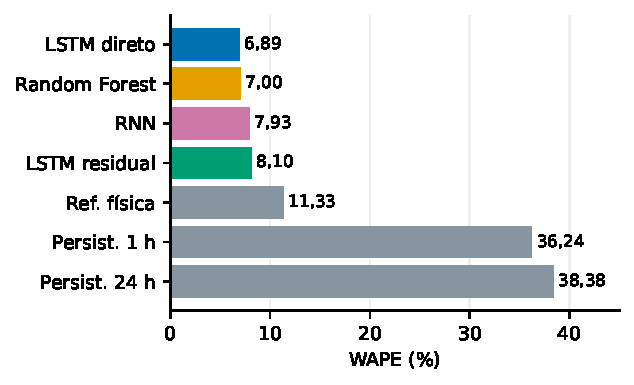
\includegraphics[width=0.75\textwidth]{imagens/fig_wape.pdf}
% \caption{Comparação do WAPE dos modelos. Fonte: resultados V3, dados sintéticos.}
% \label{fig:wape}
% \end{figure}

\begin{figure}[!h]
\centering
\textbf{Fonte:} Elaborado pelo autor.
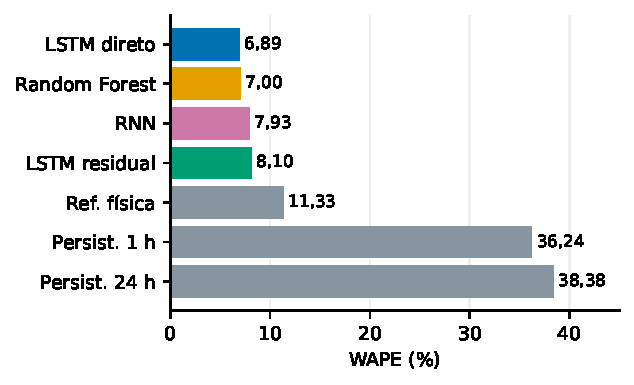
\includegraphics[width=0.75\textwidth]{imagens/fig_wape.pdf}
\caption{Comparação do WAPE dos modelos.}
\label{fig:wape}
\end{figure}

A Figura~\ref{fig:hour} apresenta o primeiro dia completo do teste, 14 de abril de 2025, para a semente 42. O total de referência foi de 28,43 kWh, enquanto o LSTM direto estimou 29,60 kWh e o Random Forest, 29,74 kWh. O gráfico apresenta previsões sucessivas de uma hora à frente, não uma previsão das 24 horas emitida de uma só vez.

\begin{figure}[H]
\centering
\textbf{Fonte:} Elaborado pelo autor.
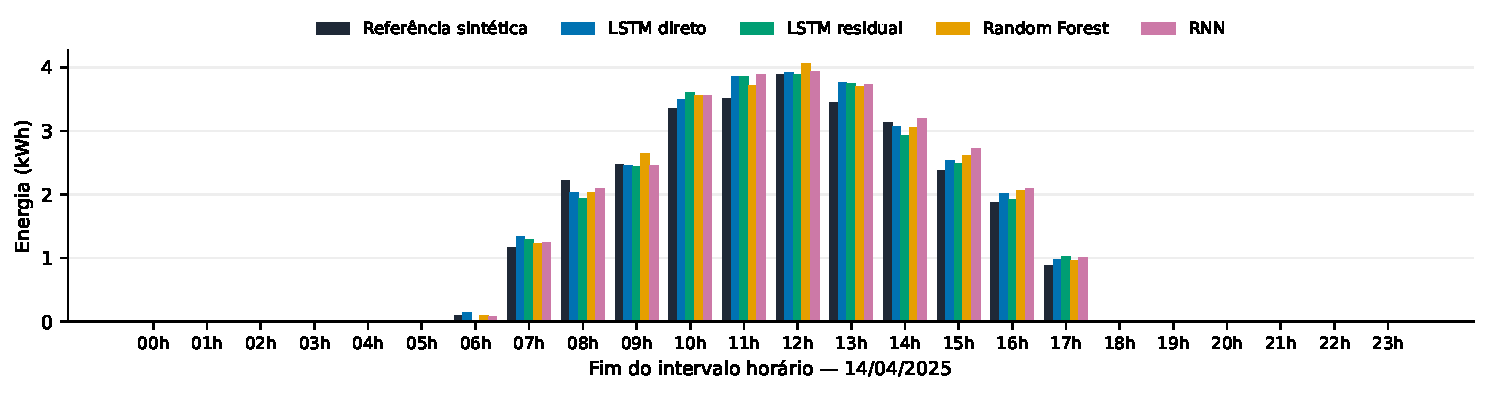
\includegraphics[width=0.99
\textwidth]{imagens/fig_24h.pdf}
\caption{Geração horária sintética e previsões em 14/04/2025, semente 42. Fonte: resultados V3.}
\label{fig:hour}
\end{figure}
% \FloatBarrier
Os resultados também foram examinados em condições meteorológicas específicas. Nos intervalos com chuva prevista, o Random Forest obteve MAE de 0,0613 kWh, ante 0,0828 kWh do LSTM direto. Sob nebulosidade prevista de pelo menos 70\%, os erros foram 0,0628 e 0,0852 kWh, respectivamente. Isso indica que a vantagem global do LSTM não se repetiu em todos os recortes. O erro médio diurno do LSTM direto foi de 0,1055 kWh, superior ao erro global, pois os 198 intervalos noturnos tiveram geração-alvo e previsões iguais a zero. Os erros de teste não constituem garantia de precisão futura.

\subsection{Relação com o estudo de Corrêa}
Em seu trabalho, Corrêa (2026, p. 54--57) \cite{correa} utilizou dados diários de geração de uma instalação do IFES em Linhares, associados à base meteorológica NSRDB. Entre quatro configurações LSTM, o modelo com variáveis meteorológicas ampliadas e codificação sazonal, com janela de três dias, apresentou MAE de 89,53 kWh e MAPE de 30,22\%. O autor observou que janelas de 30 dias não produziram os melhores resultados e discutiu a influência da quantidade e da qualidade dos dados de entrada.

Essa observação reforça a motivação para manter uma arquitetura simples e incluir informações meteorológicas e temporais relevantes neste projeto. Entretanto, os valores de erro dos dois estudos não podem ser comparados diretamente: Corrêa utilizou geração diária medida em uma instalação de porte distinto, enquanto este estudo utilizou geração horária sintética e métricas percentuais diferentes. A janela de 24 horas adotada aqui também não foi comparada com outros tamanhos neste experimento.
\section{Conclusão}
O estudo demonstrou a viabilidade de implementar um modelo de previsão fotovoltaica que combina informações meteorológicas, histórico de geração e parâmetros físicos dos equipamentos. O LSTM direto apresentou o menor erro no teste simulado, enquanto a RNN liderou a validação e o Random Forest foi competitivo, especialmente sob chuva e nebulosidade. A aprendizagem residual melhorou a estimativa física, mas não foi a abordagem mais precisa do comparativo.

Conclui-se que a seleção das variáveis, a coerência física e a avaliação dos erros são essenciais para o desenvolvimento de um projeto de Machine Learning aplicado à energia solar. A arquitetura simples é adequada como prova de conceito acadêmica. A precisão operacional e a capacidade de generalização ainda precisam ser demonstradas com medições reais.

\section{Limitações e trabalhos futuros}
A principal limitação é o uso de dados sintéticos, construídos por um processo que compartilha relações com a referência física. A meteorologia simulada não representa fielmente os erros de uma previsão operacional. Além disso, o período de 120 dias não cobre todas as estações, e o modelo físico não representa em detalhe sombreamento, falhas, indisponibilidades ou curvas reais de eficiência dos inversores. Não houve experimento isolando o efeito de cada ajuste de treinamento.

Para uma validação em Pernambuco, recomenda-se utilizar registros horários de geração AC de uma instalação real, características técnicas dos equipamentos e previsões meteorológicas emitidas antes da hora-alvo. O ONS \cite{ons} e o Open-Meteo \cite{meteo} são fontes candidatas, sujeitas à verificação de localização, unidade, granularidade e disponibilidade. O download das bases reais não foi concluído neste projeto. Também se recomenda utilizar um conjunto de teste independente, incluindo diferentes estações e condições adversas.

% \section*{Reprodutibilidade}
% O pacote V3 contém o código Python, a configuração dos equipamentos, os CSVs de entrada e de resultados, os gráficos e os pesos salvos do LSTM residual. Para reproduzir o experimento após instalar as dependências, executar:\par\noindent\texttt{python solar.py --demo --epocas 40 --seeds 42 123 2026}.

\bibliographystyle{IEEEtran}
\bibliography{referencias}

\end{document}
